\section{Phosphorescence identification on a set of ITL sensors}
\label{appendix:phos:ident}
\begin{figure}[!htbp]
\centering
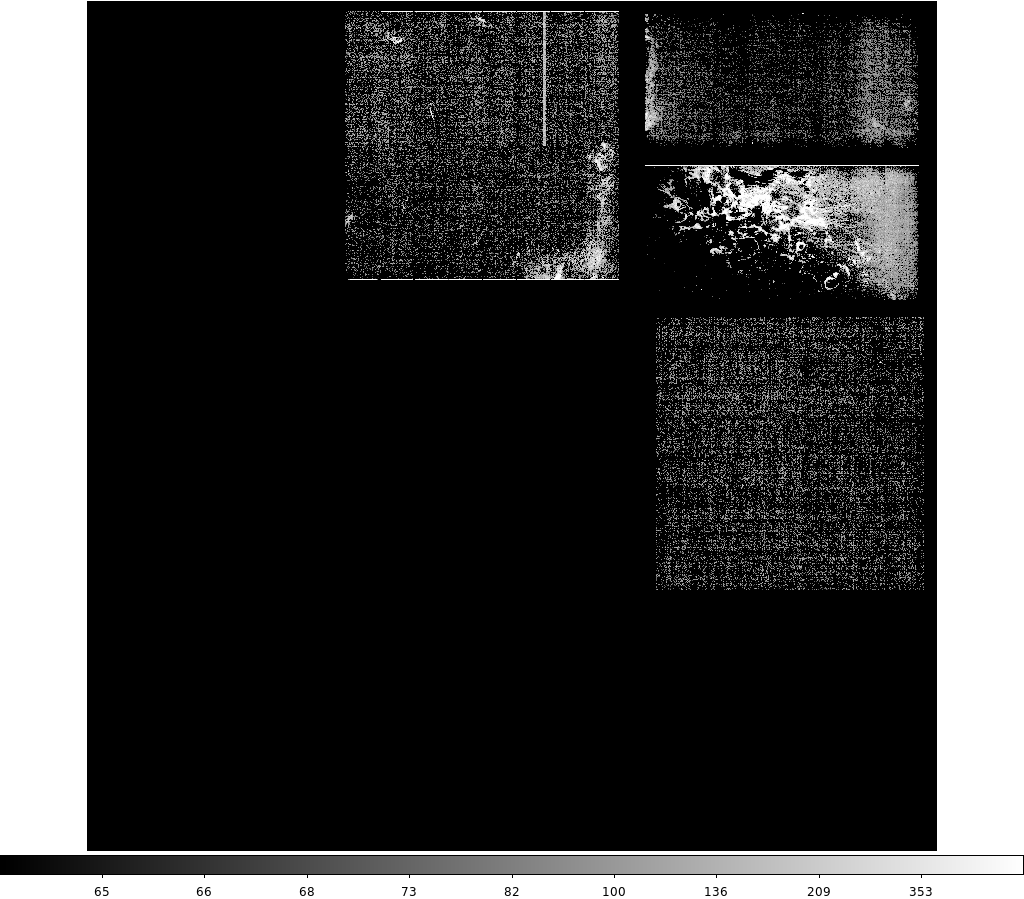
\includegraphics[width=0.9\textwidth]{figures/phosphorescence-survey/itl_fluor_R00_0-19_rb1_log.png}
\caption{Phosphorescence transients for the R00 CRTM captured in the first 15\,s following {\it red} CCOB LED at 400\,ke$^-$/pixel. With 8$\times$8 blocking, the upper end of the color scale (640) corresponds to 10\,e$^-$/pixel when averaged over 64 pixels contributing.}
\label{fig:phos:R00}
\end{figure}

\begin{figure}[!htbp]
\centering
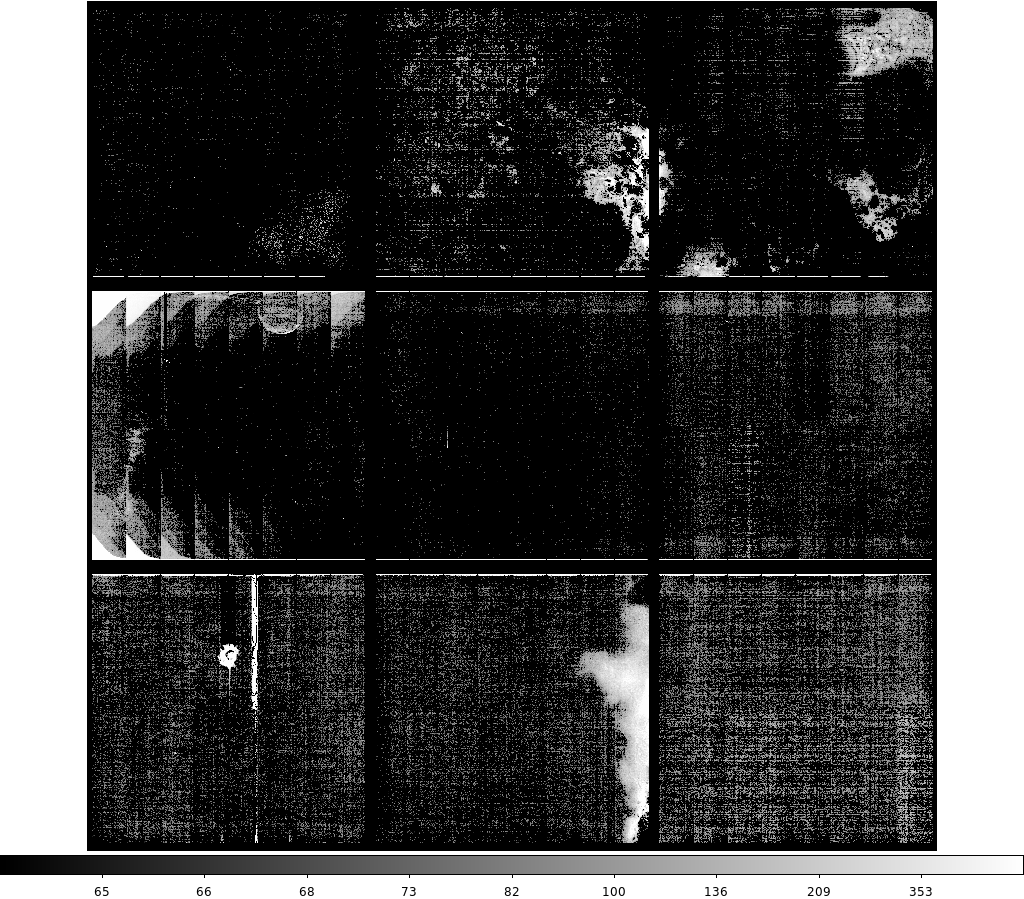
\includegraphics[width=0.9\textwidth]{figures/phosphorescence-survey/itl_fluor_R01_0-19_rb1_log.png}
\caption{Phosphorescence transients for the R01 RTM captured in the first 15\,s following {\it red} CCOB LED at 400\,ke$^-$/pixel. With 8$\times$8 blocking, the upper end of the color scale (640) corresponds to 10 e$^-$/pixel when averaged over 64 pixels contributing.}
\label{fig:phos:R01}
\end{figure}

\begin{figure}[!htbp]
\centering
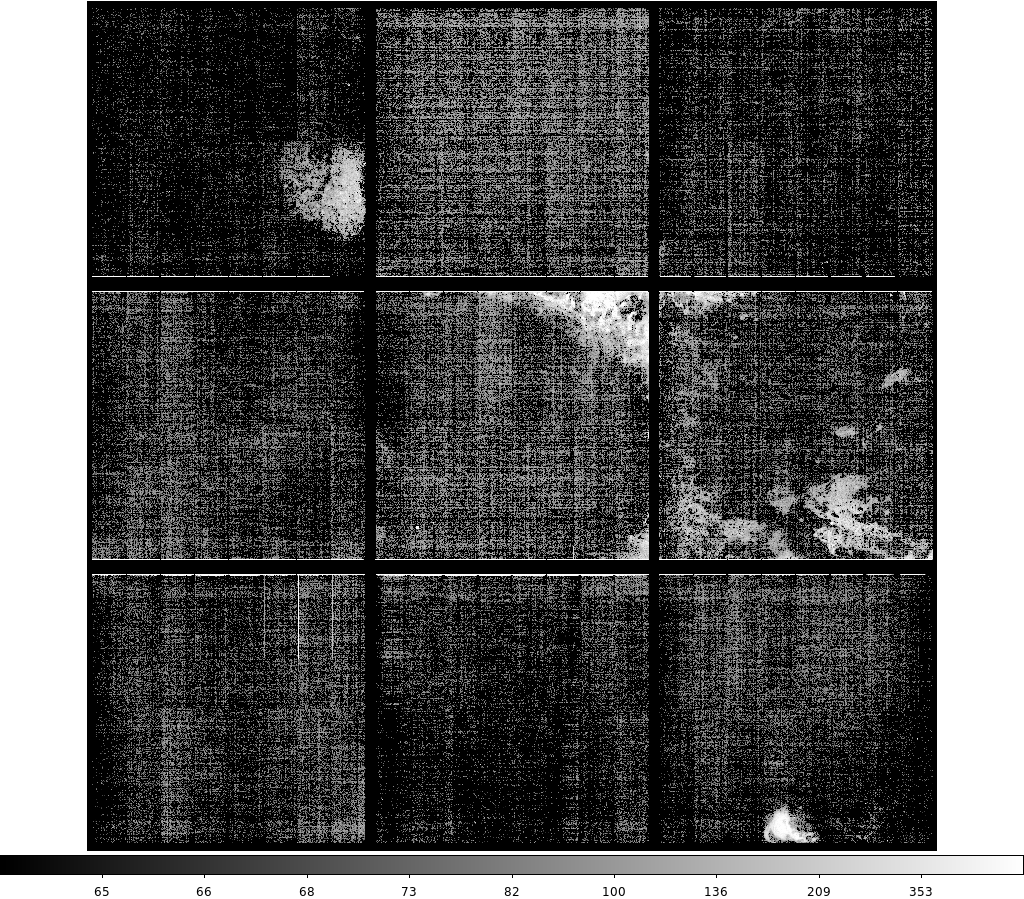
\includegraphics[width=0.9\textwidth]{figures/phosphorescence-survey/itl_fluor_R02_0-19_rb1_log.png}
\caption{Phosphorescence transients for the R02 RTM captured in the first 15\,s following {\it red} CCOB LED at 400\,ke$^-$/pixel. With 8$\times$8 blocking, the upper end of the color scale (640) corresponds to 10 e$^-$/pixel when averaged over 64 pixels contributing.}
\label{fig:phos:R02}
\end{figure}

\begin{figure}[!htbp]
\centering
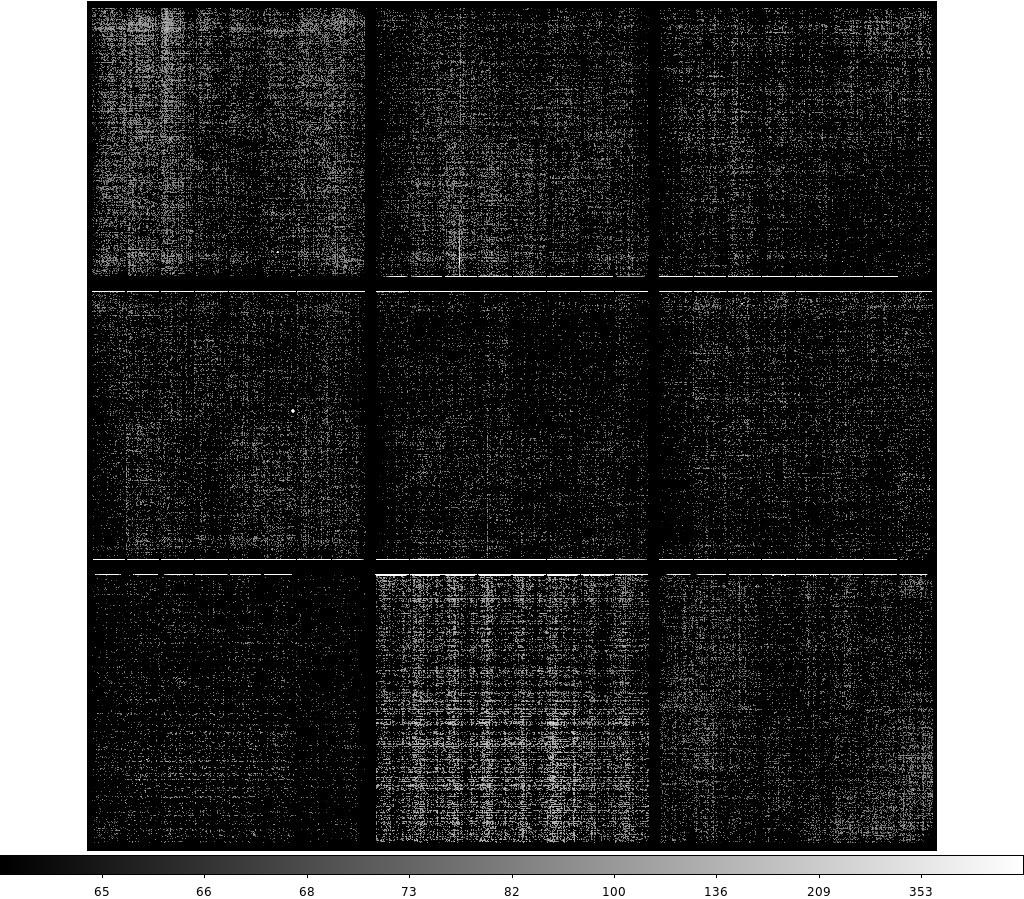
\includegraphics[width=0.9\textwidth]{figures/phosphorescence-survey/itl_fluor_R03_0-19_rb1_log.png}
\caption{Phosphorescence transients for the R03 RTM captured in the first 15\,s following {\it red} CCOB LED at 400\,ke$^-$/pixel. With 8$\times$8 blocking, the upper end of the color scale (640) corresponds to 10 e$^-$/pixel when averaged over 64 pixels contributing.}
\label{fig:phos:R03}
\end{figure}

\begin{figure}[!htbp]
\centering
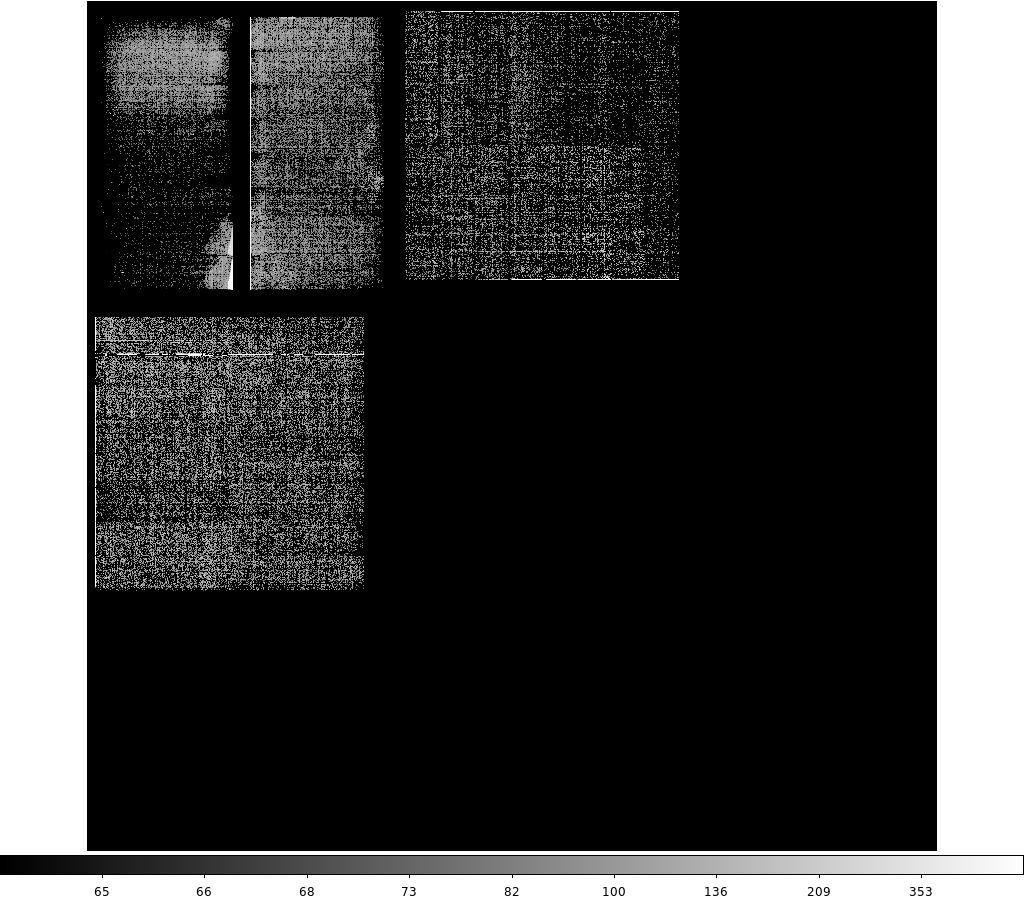
\includegraphics[width=0.9\textwidth]{figures/phosphorescence-survey/itl_fluor_R04_0-19_rb1_log.png}
\caption{Phosphorescence transients for the R04 CRTM captured in the first 15\,s following {\it red} CCOB LED at 400\,ke$^-$/pixel. With 8$\times$8 blocking, the upper end of the color scale (640) corresponds to 10 e$^-$/pixel when averaged over 64 pixels contributing.}
\label{fig:phos:R04}
\end{figure}

\begin{figure}[!htbp]
\centering
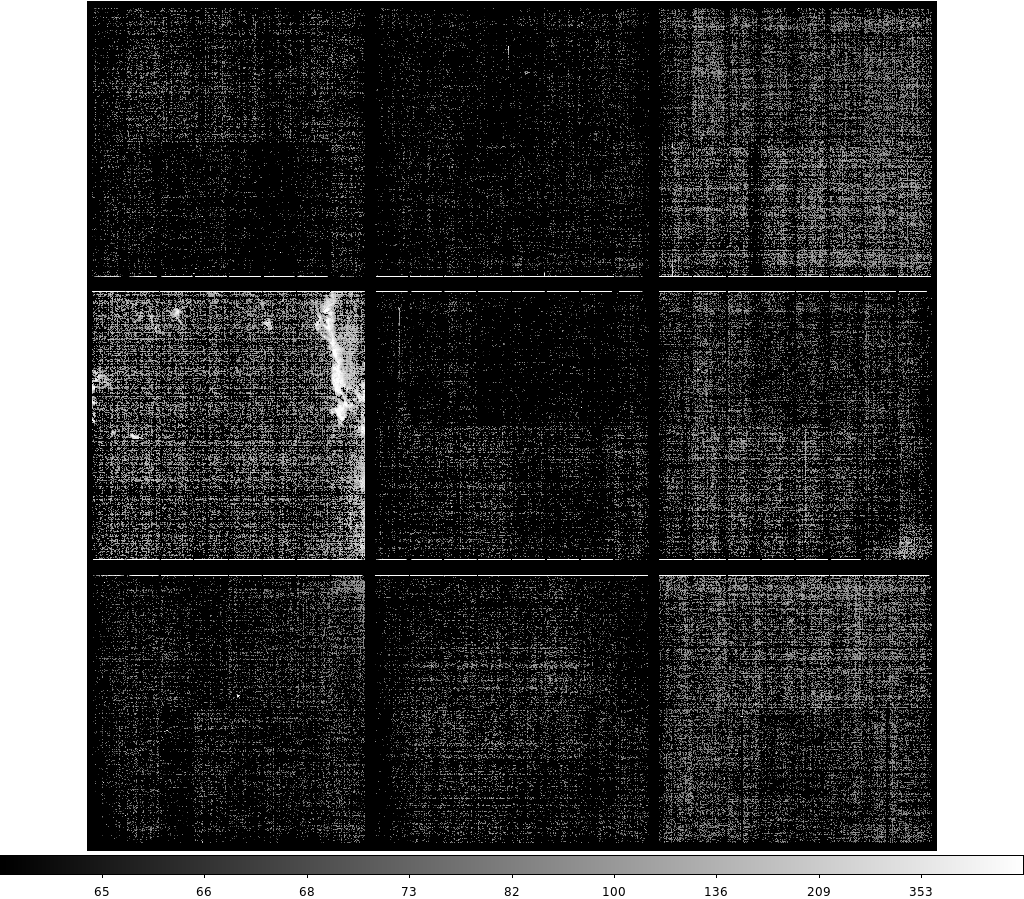
\includegraphics[width=0.9\textwidth]{figures/phosphorescence-survey/itl_fluor_R10_0-19_rb1_log.png}
\caption{Phosphorescence transients for the R10 RTM captured in the first 15\,s following {\it red} CCOB LED at 400\,ke$^-$. With 8$\times$8 blocking, the upper end of the color scale (640) corresponds to 10 e$^-$/pixel when averaged over 64 pixels contributing.}
\label{fig:phos:R10}
\end{figure}

\begin{figure}[!htbp]
\centering
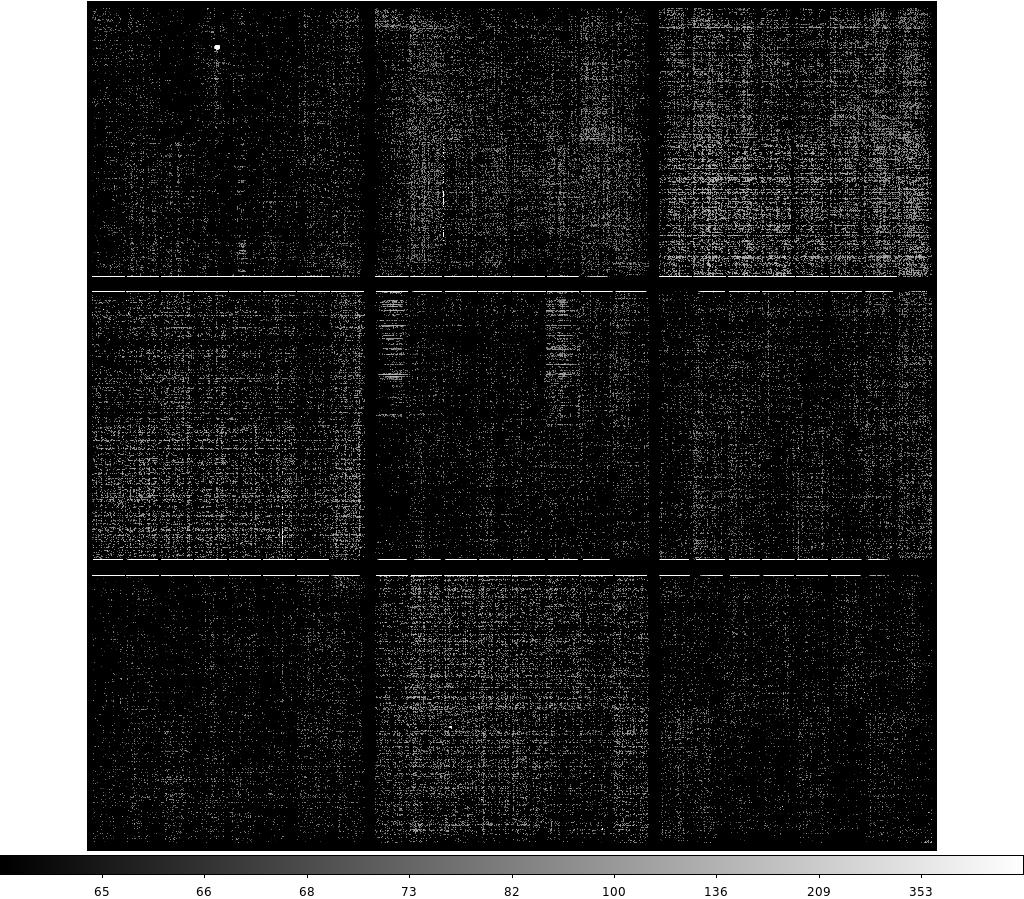
\includegraphics[width=0.9\textwidth]{figures/phosphorescence-survey/itl_fluor_R20_0-19_rb1_log.png}
\caption{Phosphorescence transients for the R20 RTM captured in the first 15\,s following {\it red} CCOB LED at 400\,ke$^-$/pixel. With 8$\times$8 blocking, the upper end of the color scale (640) corresponds to 10 e$^-$/pixel when averaged over 64 pixels contributing.}
\label{fig:phos:R20}
\end{figure}

\begin{figure}[!htbp]
\centering
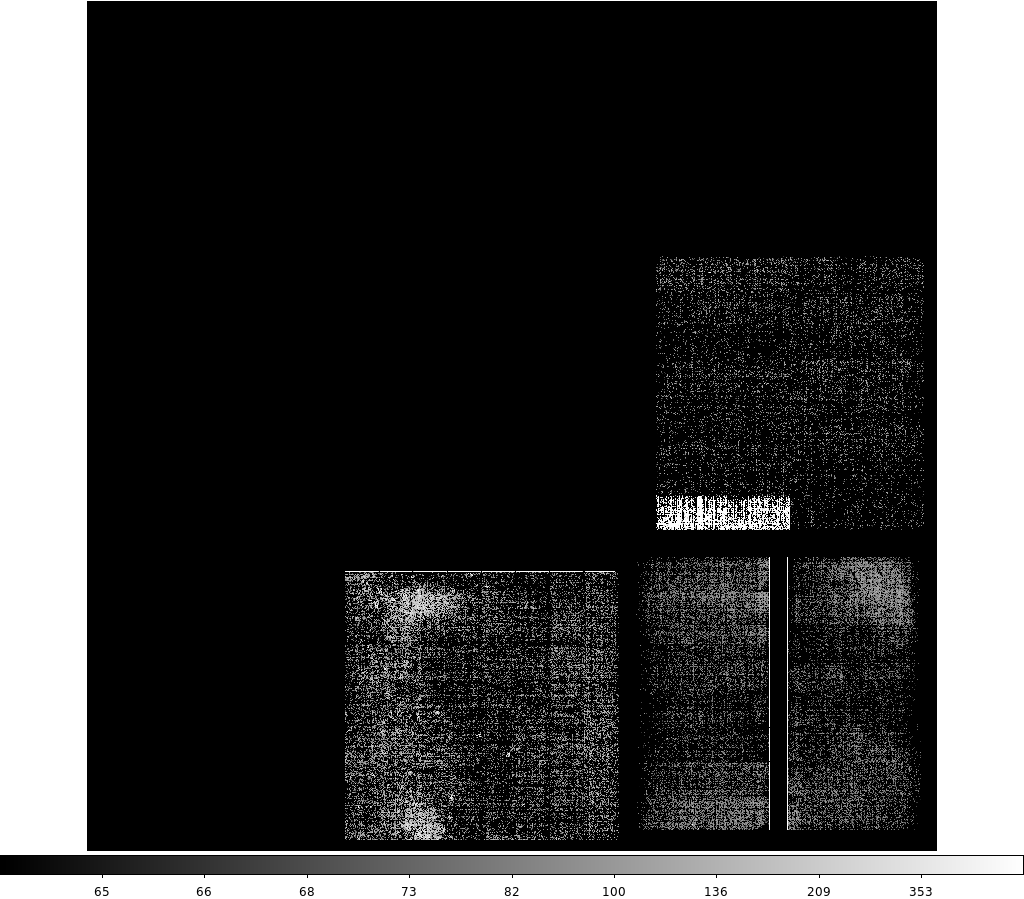
\includegraphics[width=0.9\textwidth]{figures/phosphorescence-survey/itl_fluor_R40_0-19_rb1_log.png}
\caption{Phosphorescence transients for the R40 CRTM captured in the first 15\,s following {\it red} CCOB LED at 400\,ke$^-$/pixel. With 8$\times$8 blocking, the upper end of the color scale (640) corresponds to 10 e$^-$/pixel when averaged over 64 pixels contributing.}
\label{fig:phos:R40}
\end{figure}

\begin{figure}[!htbp]
\centering
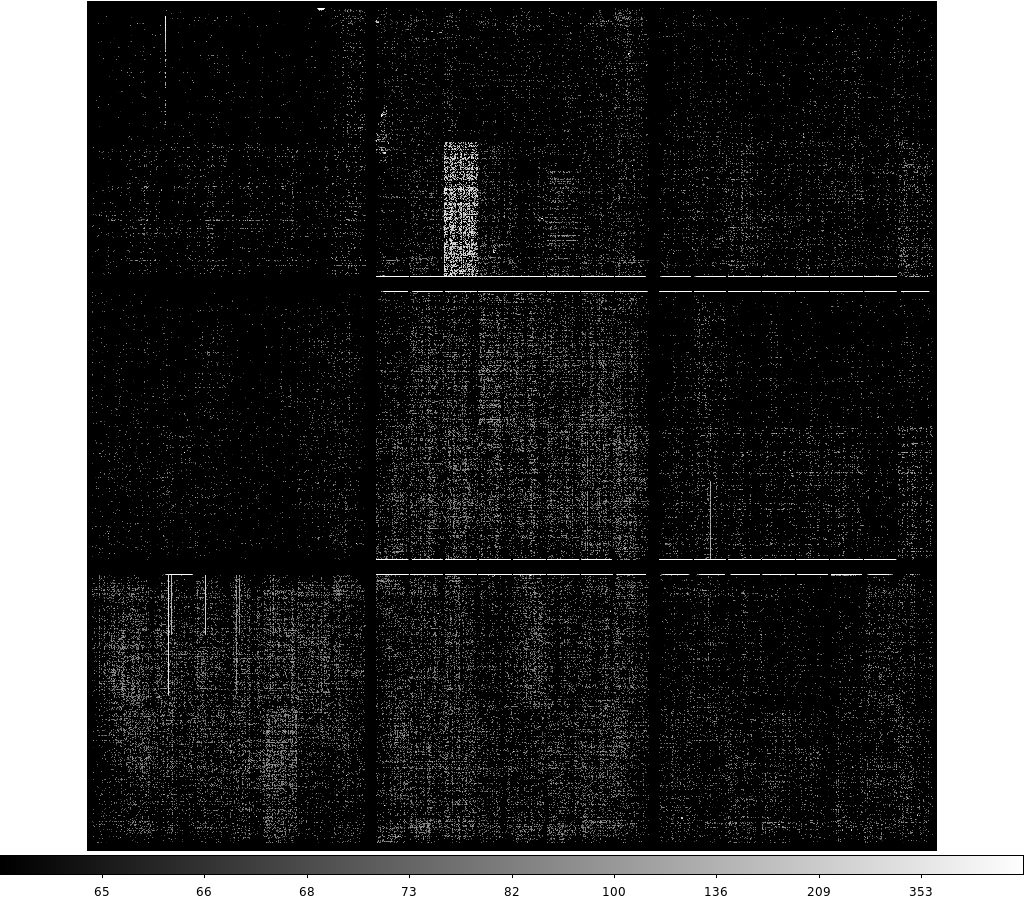
\includegraphics[width=0.9\textwidth]{figures/phosphorescence-survey/itl_fluor_R41_0-19_rb1_log.png}
\caption{Phosphorescence transients for the R41 RTM captured in the first 15\,s following {\it red} CCOB LED at 400\,ke$^-$/pixel. With 8$\times$8 blocking, the upper end of the color scale (640) corresponds to 10 e$^-$/pixel when averaged over 64 pixels contributing.}
\label{fig:phos:R41}
\end{figure}

\begin{figure}[!htbp]
\centering
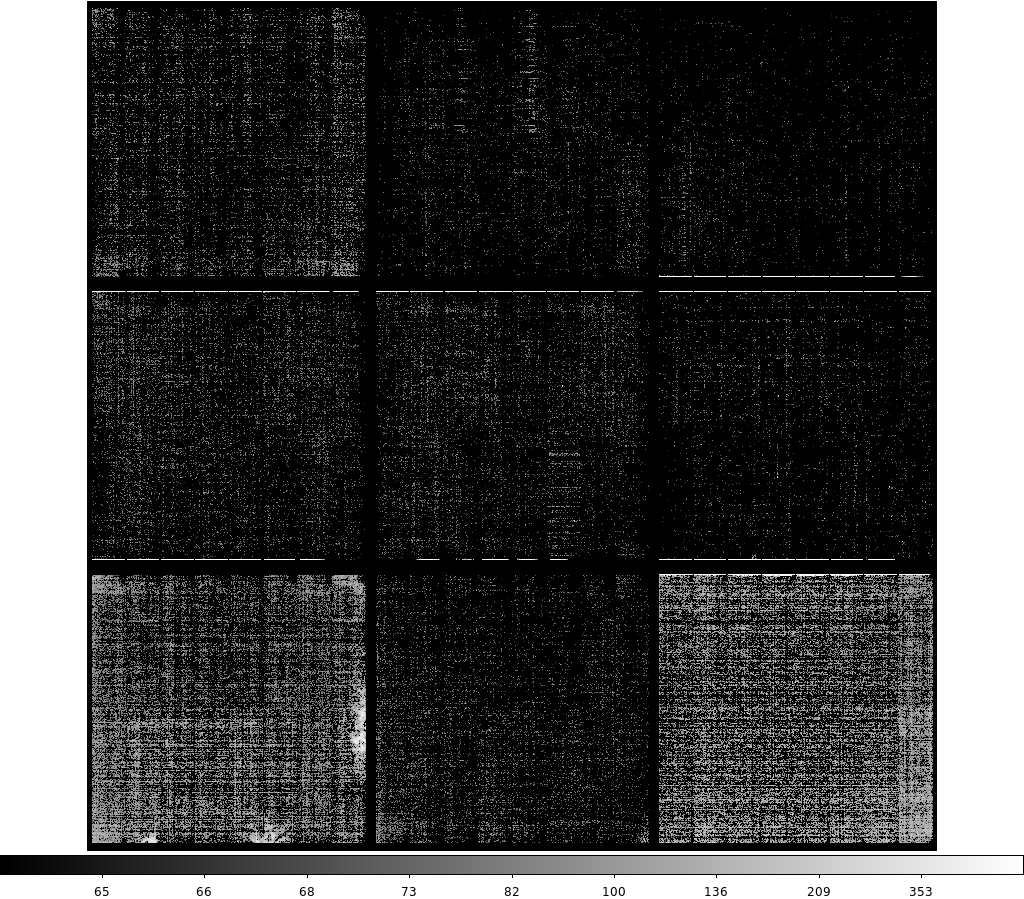
\includegraphics[width=0.9\textwidth]{figures/phosphorescence-survey/itl_fluor_R42_0-19_rb1_log.png}
\caption{Phosphorescence transients for the R42 RTM captured in the first 15\,s following {\it red} CCOB LED at 400\,ke$^-$/pixel. With 8$\times$8 blocking, the upper end of the color scale (640) corresponds to 10 e$^-$/pixel when averaged over 64 pixels contributing.}
\label{fig:phos:R42}
\end{figure}

\begin{figure}[!htbp]
\centering
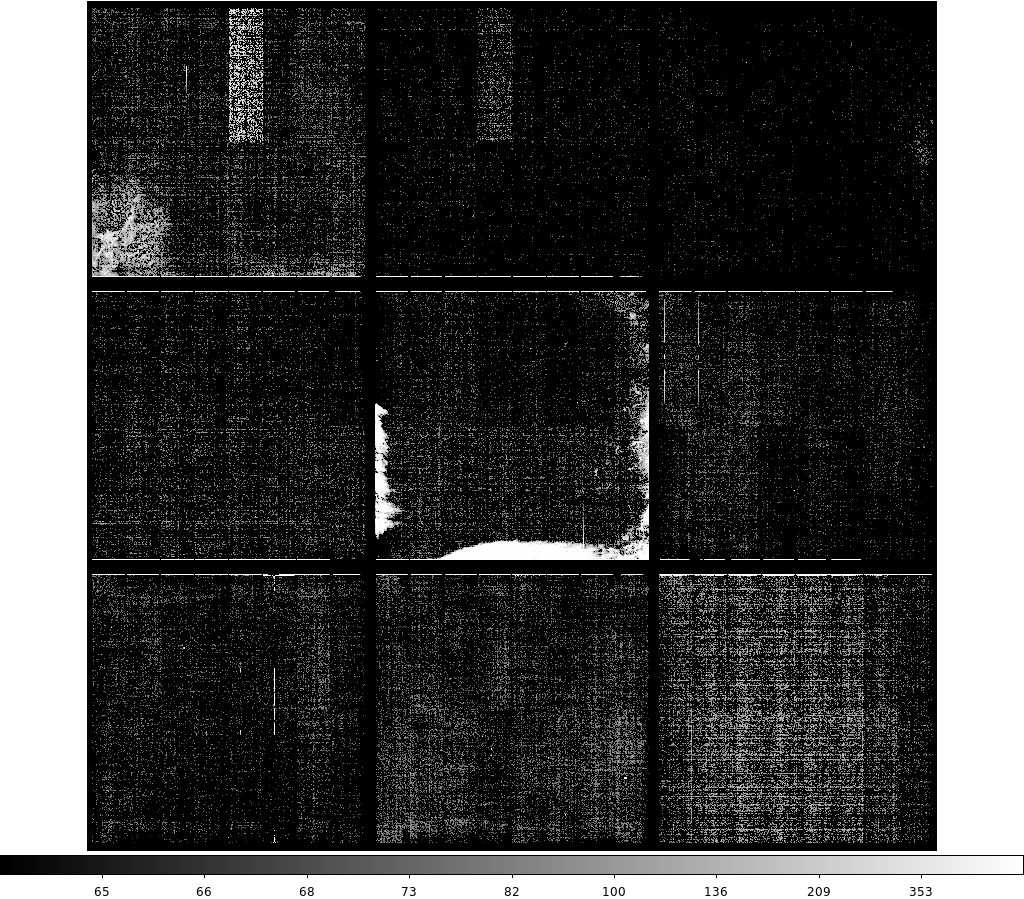
\includegraphics[width=0.9\textwidth]{figures/phosphorescence-survey/itl_fluor_R43_0-19_rb1_log.png}
\caption{Phosphorescence transients for the R43 RTM captured in the first 15\,s following {\it red} CCOB LED at 400\,ke$^-$/pixel. With 8$\times$8 blocking, the upper end of the color scale (640) corresponds to 10 e$^-$/pixel when averaged over 64 pixels contributing.}
\label{fig:phos:R43}
\end{figure}

\begin{figure}[!htbp]
\centering
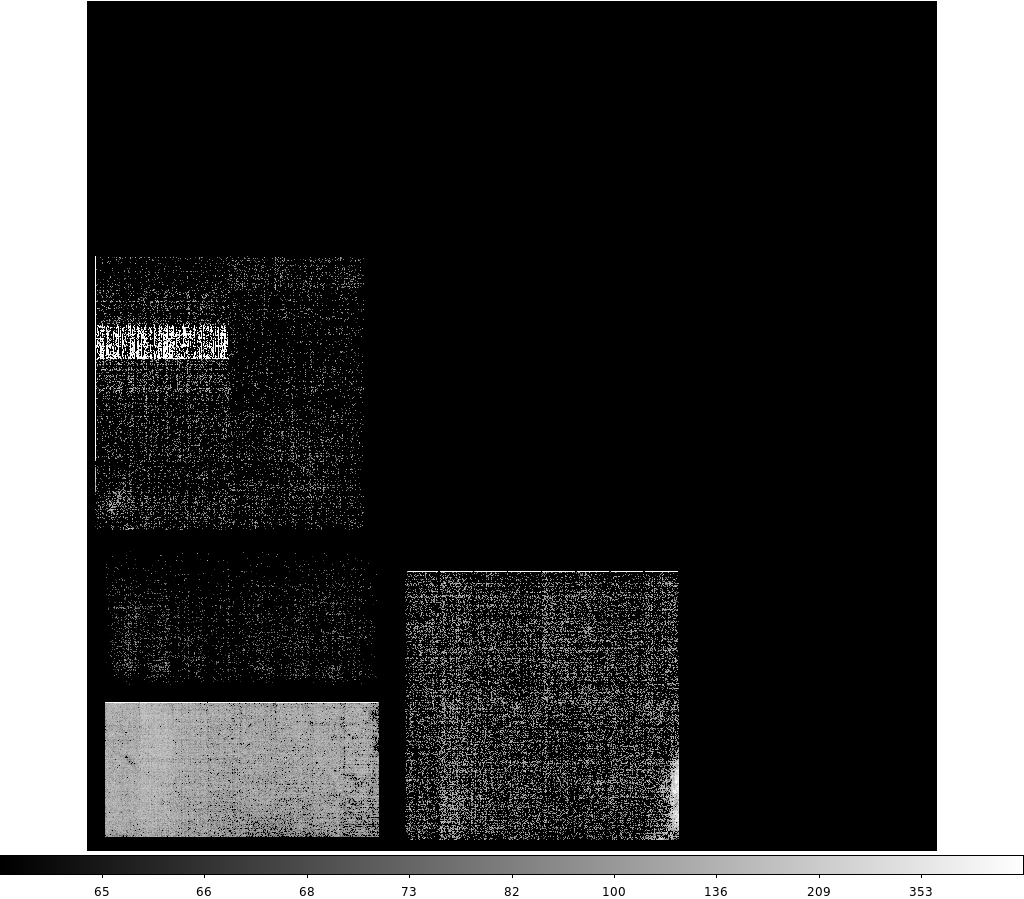
\includegraphics[width=0.9\textwidth]{figures/phosphorescence-survey/itl_fluor_R44_0-19_rb1_log.png}
\caption{Phosphorescence transients for the R44 CRTM captured in the first 15\,s following {\it red} CCOB LED at 400\,ke$^-$/pixel. With 8$\times$8 blocking, the upper end of the color scale (640) corresponds to 10 e$^-$/pixel when averaged over 64 pixels contributing.}
\label{fig:phos:R44}
\end{figure}
